\subsection{Du perceptron au réseau de neurones}

\begin{frame}{Le neurone}
	\begin{block}{Présentation du modèle du perceptron}
		En 1943, McCulloch et Pitts introduisent le modèle du perceptron.  \\
		Ce modèle est basé sur le fonctionnement du neurone humain.
	\end{block}
	\begin{figure}
		\centering
		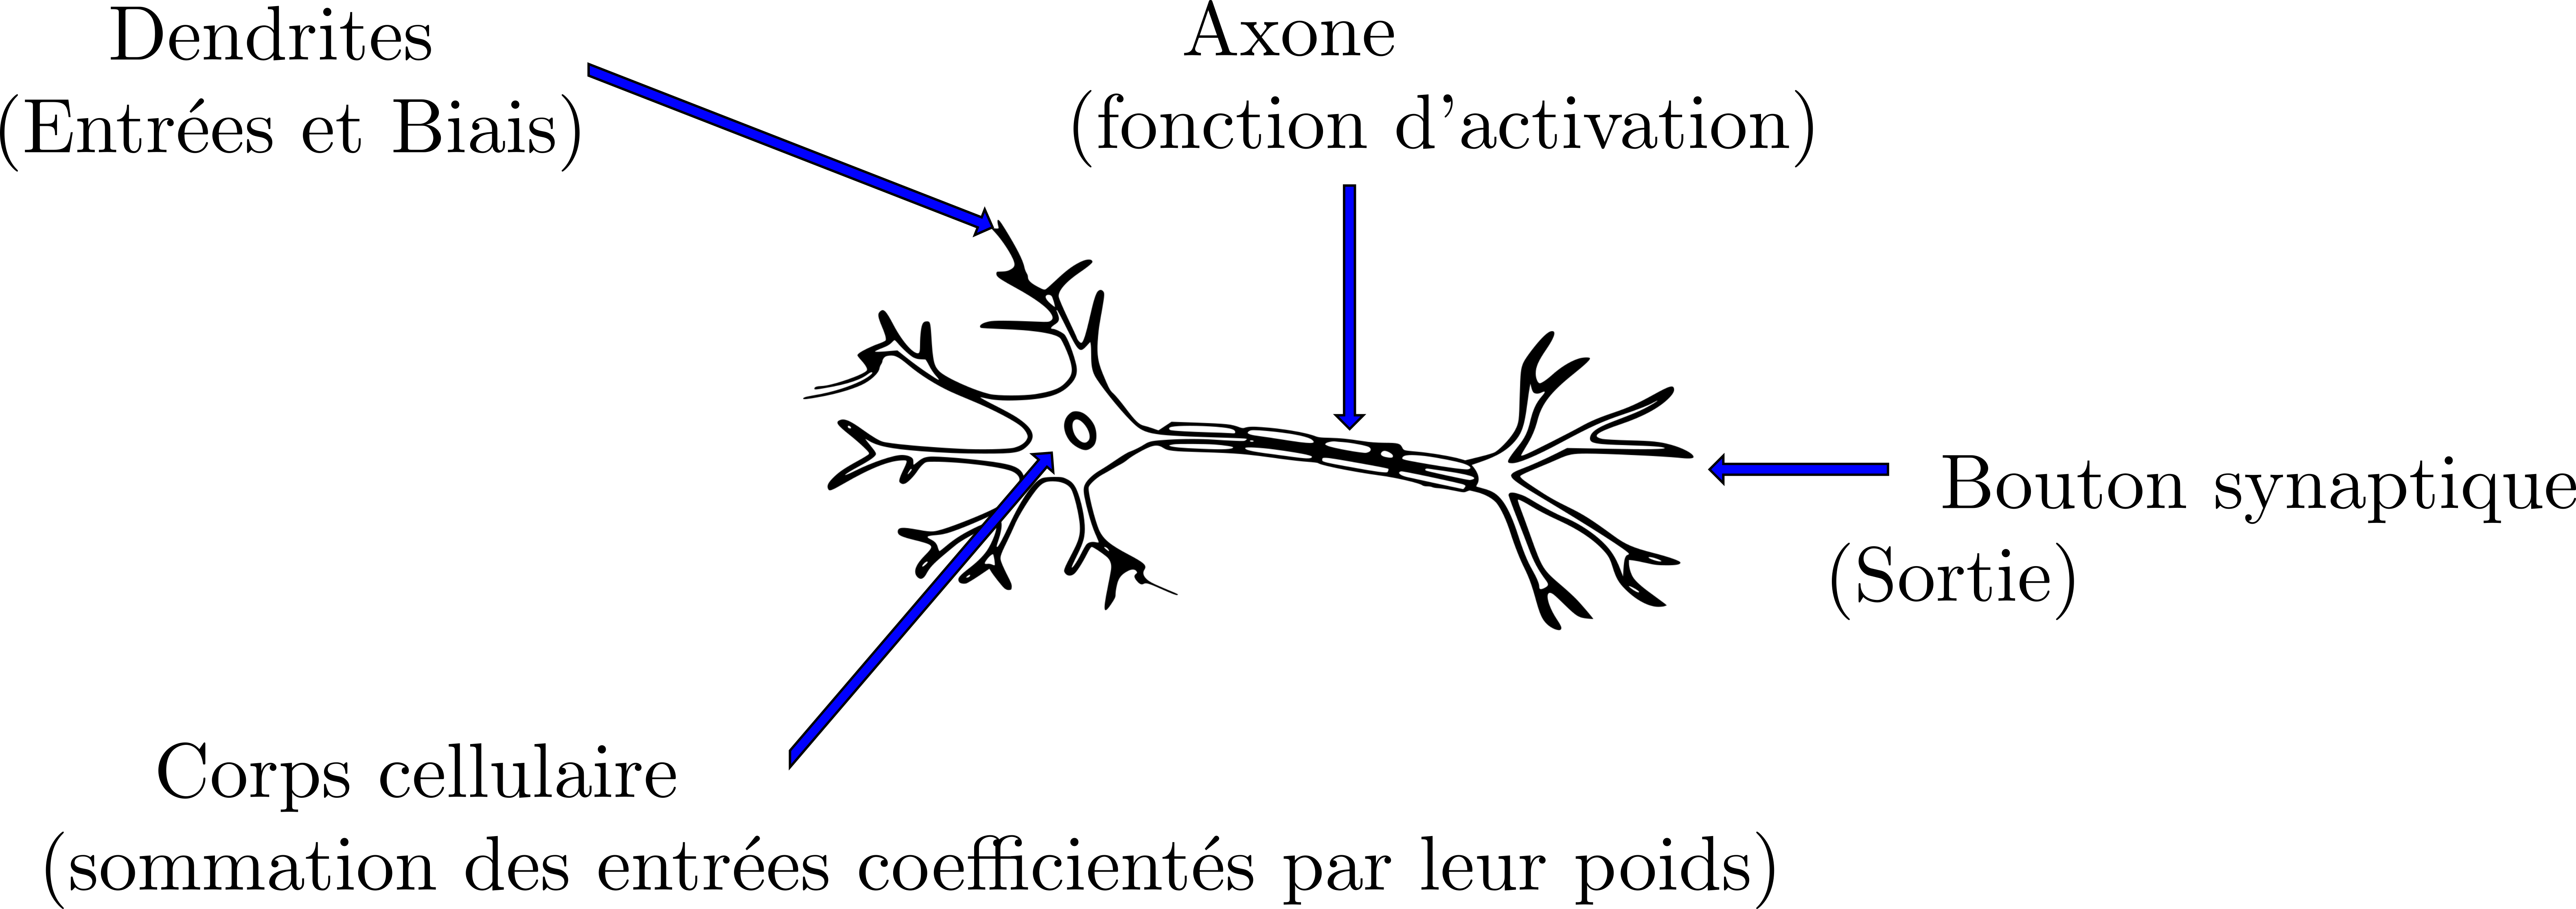
\includegraphics[width=\textwidth]{2-Neurone.png}
		\caption{Schéma d'un neurone humain}
	\end{figure}
\end{frame}

\begin{frame}{Le perceptron}
	\begin{figure}
		\centering
		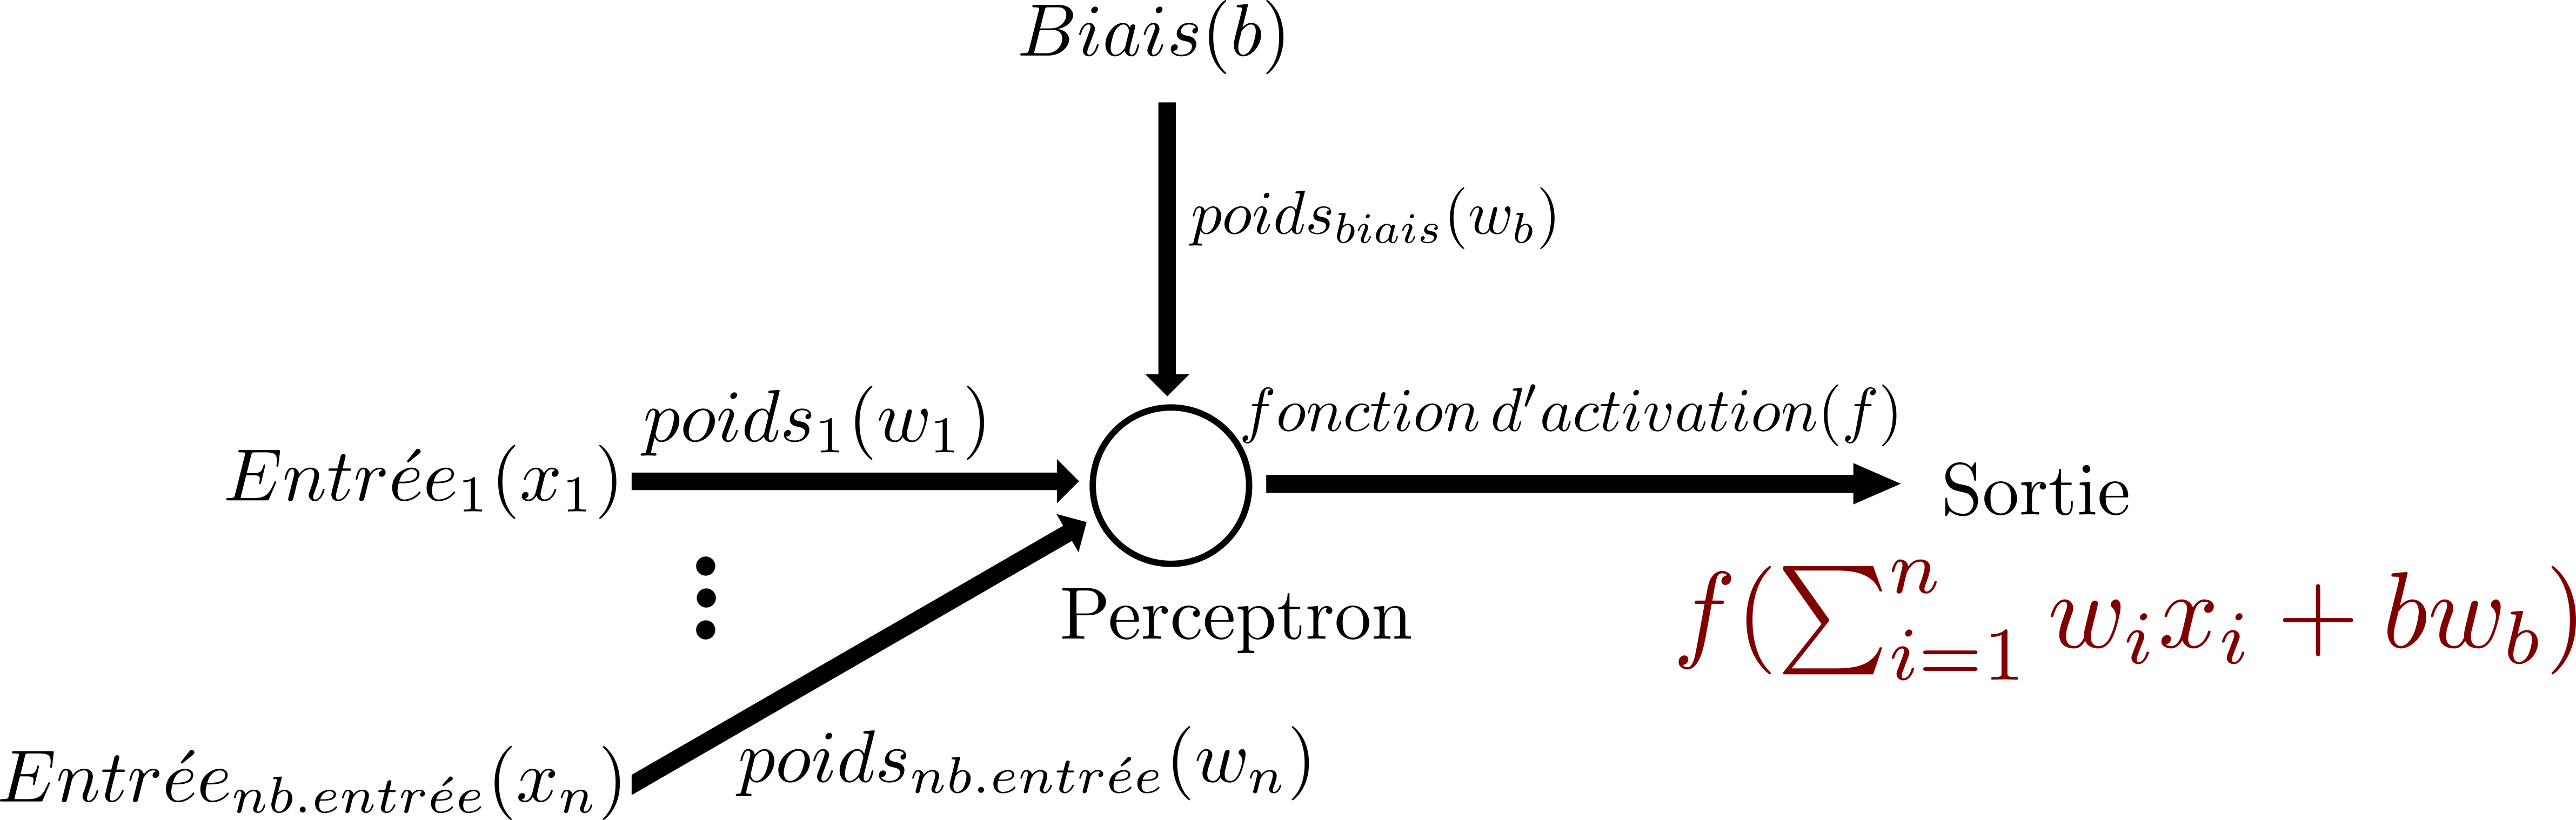
\includegraphics[width=\textwidth]{1-Perceptron.png}
		\caption{Schéma d'un perceptron}
	\end{figure}
\end{frame}


\begin{frame}{Sa représentation informatique}
	\begin{columns}
		\begin{column}[]{0.4\textwidth}
			\begin{center}
				$
					f
					\left(
					\begin{pmatrix}
						x_1 & \ldots & x_n & b
					\end{pmatrix}
					\times
					\begin{pmatrix}
						w_1    \\
						\vdots \\
						w_n    \\
						w_b
					\end{pmatrix}
					\right)
				$ \\
			\end{center}
		\end{column}
		\begin{column}[]{0.5\textwidth}
			\lstinputlisting[language=Python, firstline=15]{0-representation.py}
		\end{column}
	\end{columns}
\end{frame}


\begin{frame}{La fonction d'activation Sigmoïde}
    \begin{center}
        \centering
		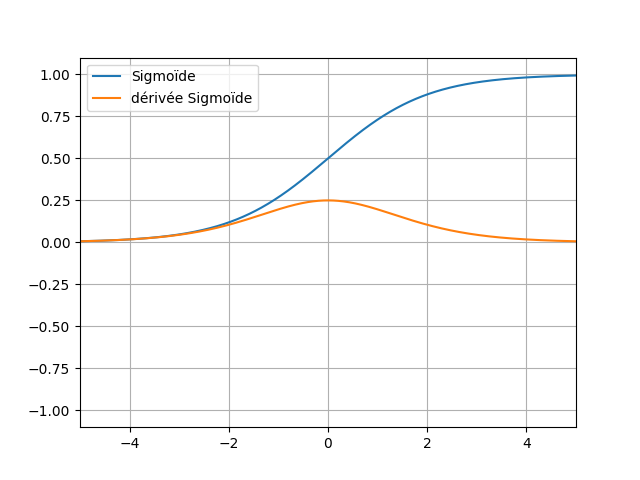
\includegraphics[width=200px]{0-Sigmoide.png} \\~\\
        Sigmoïde : $\mathlarger{\frac{1}{1+e^{-x}}}$ \\~\\
        Dérivée : $f(x) \times (1-f(x))$
    \end{center}   
\end{frame}

\begin{frame}{Le réseau de neurones}
    \begin{figure}
        \centering
        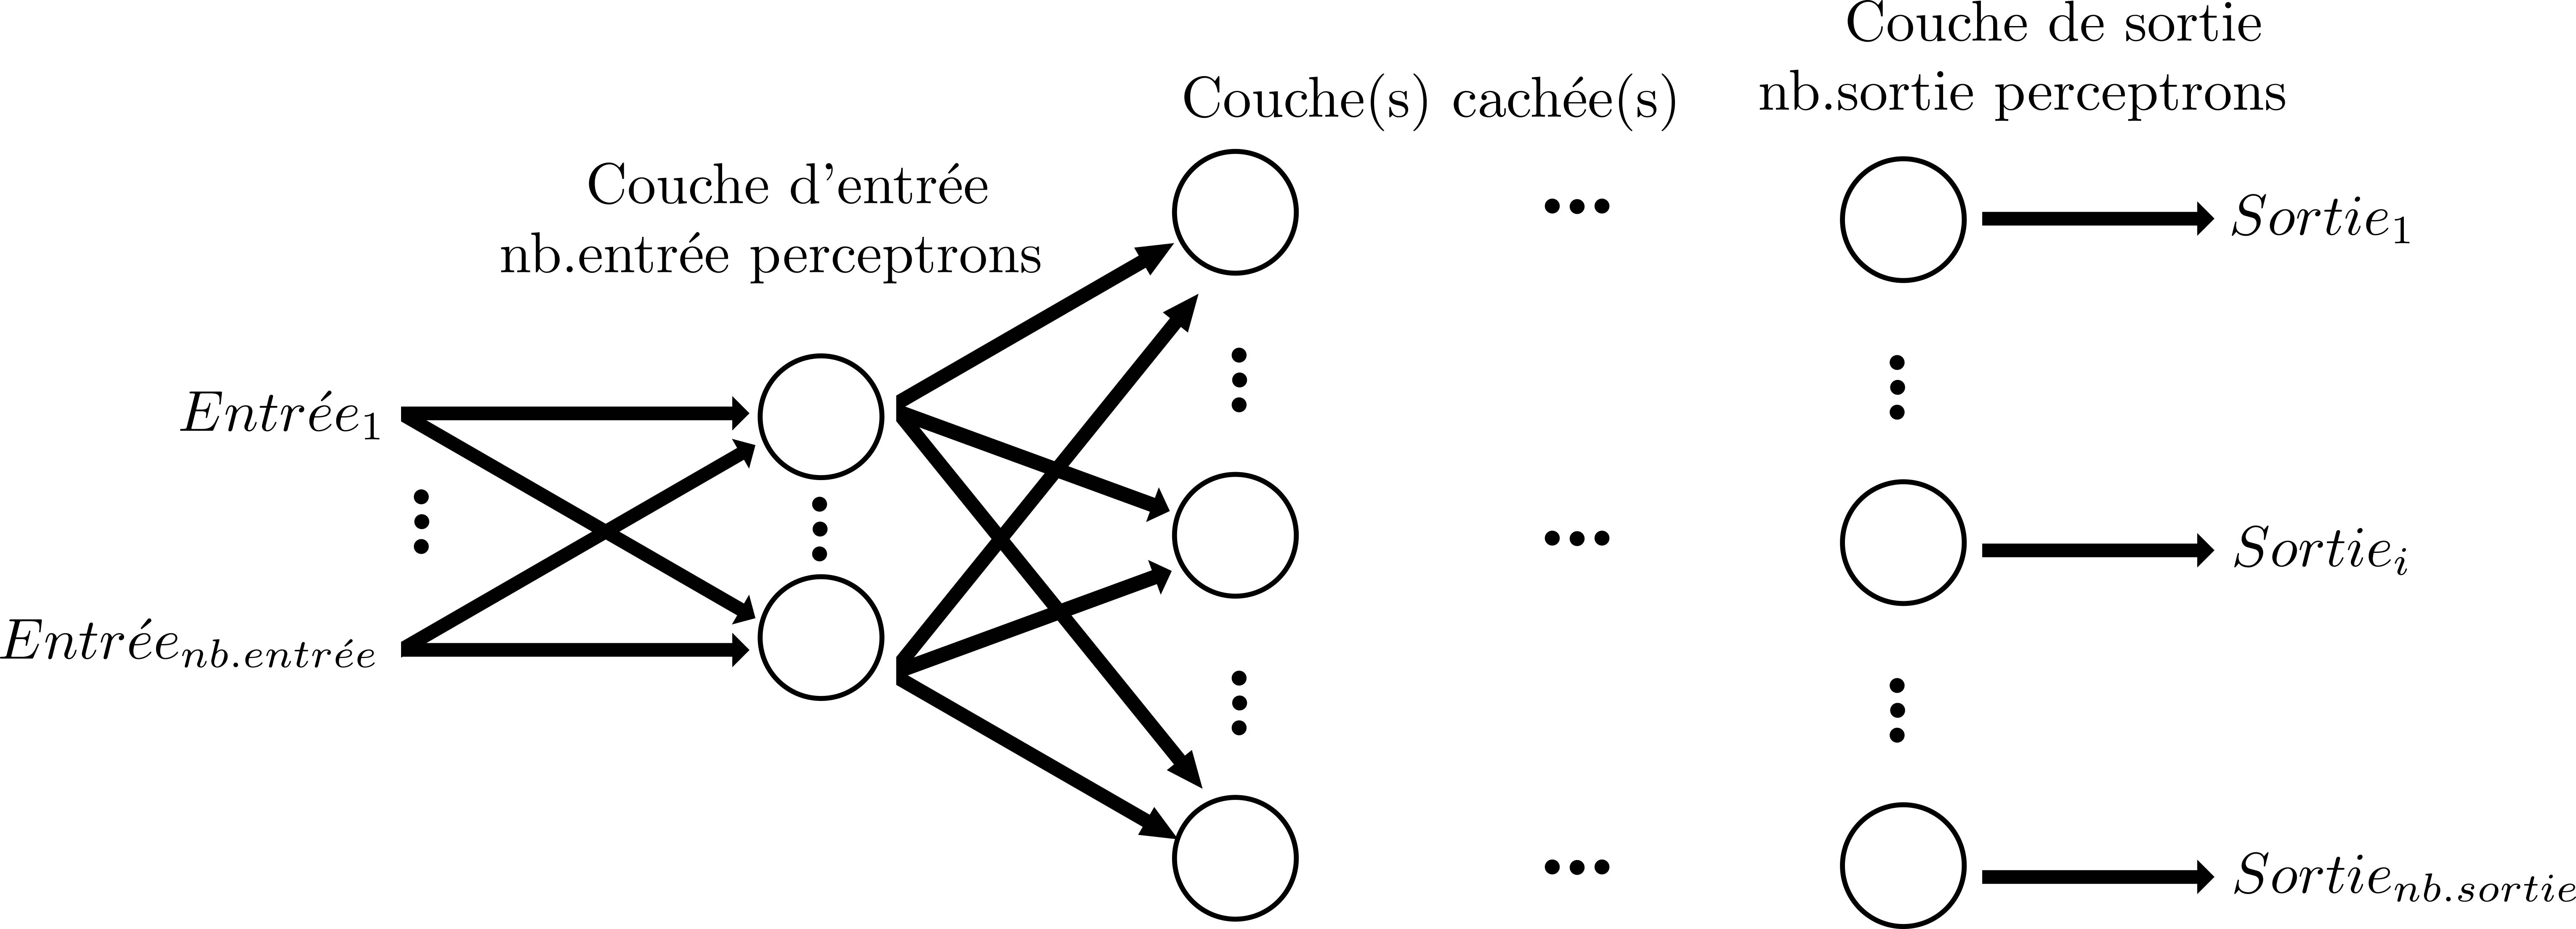
\includegraphics[width=\textwidth]{3-Reseau}
        \caption[]{Schéma d'un réseau de neurones}
    \end{figure}
\end{frame}